\centerline{\bf \Huge Финальная МатДрака }

\problem{\textbf{1!}} Чётно или нечётно число  1 + 2 + 3 + ... + 2025?


\problem{\textbf{2}} Сумму цифр шестизначного числа умножили на произведение его цифр. Получилось 390. Найдите хотя бы одно такое шестизначное число.

\problem{\textbf{3}} Сколько целых чисел от 378 до 2433 имеют сумму цифр, делящуюся
на 5?


\problem{\textbf{4}} Незнайка лжёт по понедельникам, вторникам и пятницам, а в остальные дни недели говорит правду. В какие дни недели Незнайка может сказать: «Я лгал позавчера и буду лгать послезавтра»?


\problem{\textbf{5}} В тёмной комнате на полке в беспорядке лежат четыре пары носков двух разных размеров и двух разных цветов. Какое наименьшее число носков необходимо, не выходя из комнаты, переложить с полки в чемодан, чтобы в нем оказались две пары различного размера и цвета?


\problem{\textbf{6}} Трое играют в настольный теннис, причем игрок, проигравший партию, уступает место игроку, не участвовавшему в ней. В итоге оказалось, что первый игрок сыграл 10 партий, второй – 21. Сколько партий сыграл третий игрок?


\problem{\textbf{7}} На сколько сумма $2^2+4^2+6^2+\ldots+100^2$ больше суммы $1^2+3^2+5^2+\ldots+99^2 ?$


\problem{\textbf{8}} Начальник записал несколько простых чисел, использовав ровно по одному
разу все цифры от 1 до 9. Сумма этих простых чисел оказалась равной 225. Можно ли, использовав ровно по одному разу те же цифры, записать несколько простых чисел так, чтобы
их сумма оказалась меньше?


\problem{\textbf{9}} Найдите количество четырёхзначных чисел, у которых третья цифра
меньше четвёртой на 2.


\problem{\textbf{10}} Каждый ученик класса - может быть девочкой, блондином или математиком. В классе 20 девочек, из них 12
блондинок, но одна блондинка математик. Всего в классе 24 ученика - блондина, среди них математиков 12, а всего
математиков (мальчиков и девочек) 17, из них 6 девочек. Сколько учеников в данном классе?


\problem{\textbf{11}} 
Разделите число 80 на две части так, чтобы одна часть составляла 60 процентов от другой части.



\newpage
\hspace{6mm}

\problem{\textbf{12}} Каких целых чисел от 1 до 60 000 (включительно) больше и на сколько: содержащих в своей записи только чётные цифры или содержащих в своей записи только
нечётные цифры?

\problem{\textbf{13}} Сколько натуральных чисел, делящихся на 4 и
меньших 1000, не содержат в десятичной записи ни одной из цифр 3, 4, 5, 7 и 9?



\problem{\textbf{14}} По кругу лежат 100 пирожков, из них 53 с капустой, а остальные — с рисом. Алексей знает, какие из них с чем, и хочет выбрать 67 подряд лежащих пирожков
так, чтобы среди них было ровно $k$ с капустой. При каких $k$ ему это гарантированно удастся сделать независимо от расположения пирожков? 

\problem{\textbf{15}} Комплект косточек домино выложен в виде прямоугольника 8×7 клеток. Попробуйте определить, как расположены косточки?

\begin{center}
    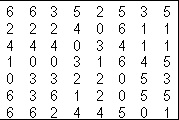
\includegraphics[width=0.4\textwidth]{Сборы/Сборы Элиста 2025/АА/7/91МатдракаII/Матдрака_15.png}
\end{center}

